\documentclass[11pt]{scrartcl}

\usepackage[sexy]{evan}
\usepackage{import}
\usepackage[table]{xcolor}
\usepackage{xfp}

\newcommand{\gad}{\textcolor{yellow}{$\bigstar$}}
\newcommand{\bad}{\textcolor{red}{$\bigstar$}}

\definecolor{dcol0}{HTML}{C8E6C9}
\definecolor{dcol1}{HTML}{D4E9B3}
\definecolor{dcol2}{HTML}{E5ED9A}
\definecolor{dcol3}{HTML}{FFF59D}
\definecolor{dcol4}{HTML}{FFE082}
\definecolor{dcol5}{HTML}{FFCC80}
\definecolor{dcol6}{HTML}{FFAB91}
\definecolor{dcol7}{HTML}{F49890}
\definecolor{dcol8}{HTML}{E57373}
\definecolor{dcol9}{HTML}{D32F2F}

\makeatletter
\newcommand{\getcolorname}[1]{dcol#1}
\makeatother

\newcommand{\dif}[1]{%
    \edef\colorindex{\number\fpeval{floor(#1)}}%
    \edef\fulltext{#1}%
    \colorbox{\getcolorname{\colorindex}}{%
        \ifnum\colorindex>8
            \textbf{\textcolor{white}{\,\fulltext\,}}%
        \else
            \textbf{\textcolor{black}{\,\fulltext\,}}%
        \fi
    }%
}
% Variable para dificultad (inicial 0)
\newcommand{\thmdifficulty}{0}

% Comando para asignar dificultad antes del problema
\newcommand{\problemdiff}[1]{\renewcommand{\thmdifficulty}{#1}}

% Estilo del problema que incluye dificultad antes del título
\declaretheoremstyle[
    headfont=\color{blue!40!black}\normalfont\bfseries,
    headformat={%
      \dif{\thmdifficulty}\quad \NAME~\NUMBER\ifx\relax\EMPTY\relax\else\ \NOTE\fi
    },
    postheadspace=1em,
    spaceabove=8pt,
    spacebelow=8pt,
    bodyfont=\normalfont
]{problemstyle}

    \declaretheorem[style=problemstyle,name=Problema,sibling=theorem]{problema}
    \declaretheorem[style=problemstyle,name=Problema,numbered=no]{problema*}

\definecolor{yellow4}{RGB}{255, 206, 0}

\title {Homotecia y 9 puntos}

\author{Emmanuel Buenrostro}


\begin{document}
\maketitle

\section{¿Qué es?}



\begin{definition}
    Una homotecia es una transofrmación de plano en la cual tienes un centro $O$ y una constante real $c\neq0$, 
    en la cual cada punto $P$ del plano, lo envia a un punto $P'$ tal que $OP'=OP\cdot c$ y $O,P,P'$ son colineales.
    \begin{center}
        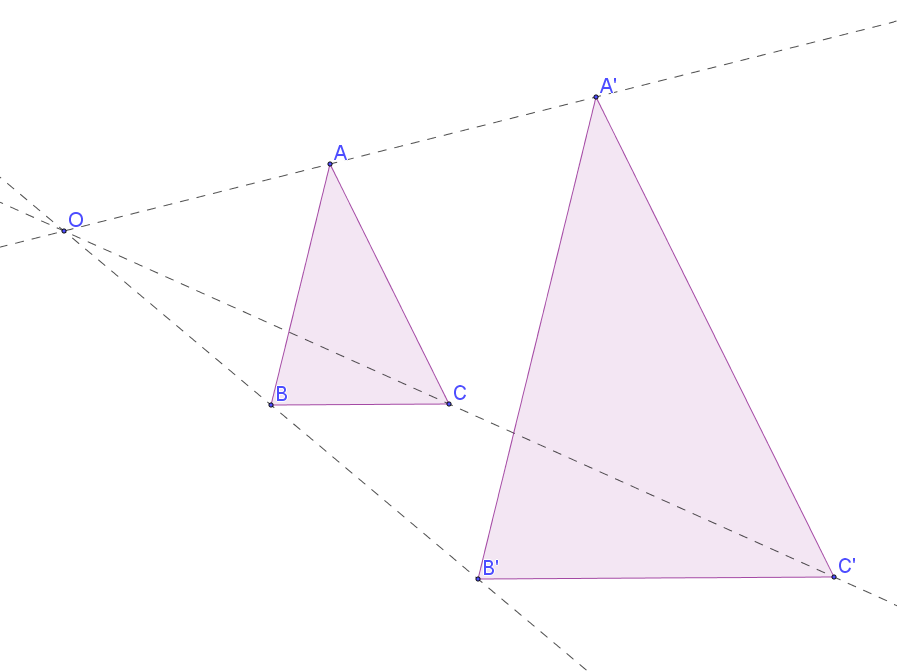
\includegraphics[scale=0.7]{Hom1.png}
    \end{center}

\end{definition}



\subsection{Propiedades:}
\begin{enumerate}
    \item $AB \parallel A'B'$
    \item $\angle ABC=\angle A'B'C'$.
    \item $A'B'C'$ es semejante a $ABC$.  (Esto aplica para cualquier figura).
    \item $A,B,C$ son colineales si y solo si $A',B',C'$ son colineales.
    \item $\ell_1, \ell_2, \ell_3$ son rectas que concurren si y solo si  $\ell_1', \ell_2', \ell_3'$ también.
    \item $\ell$ es tangente a $\Gamma$ en $T$, si y solo si $\ell'$ es tangente a $\Gamma'$ en el punto $T'$.
    \item $ABCD$ es ciclico si y solo si  $A'B'C'D'$ es ciclico (Esto en realidad hace que los circulos se van a otros circulos).
    \item $\ell_1, \ell_2 $ son paralelas si y solo si $\ell_1', \ell_2'$.
    \item $\ell_1, \ell_2$ son perpendiculares si y solo si $\ell_1', \ell_2'$ son perpendiculares.
\end{enumerate}
Porque el enfasis en el si y solo si, ya que en varios problemas ocupas usar homotecia, lo que haces es probar una propiedad para alguno de los dos, y luego usarla en el otro lado de la homotecia.  \\

Para probar el primer punto, es un Tales. \\

Para probar el segundo punto 




Ahora, no siempre tenemos un centro "directo" de homotecia, a veces tenemos que construirlo. \\

Un caso especial es saber cuando dos triangulos tienen un centro de homotecia. \\

Primero, que necesitamos para que si tienes dos triangulos $ABC, A'B'C$ exista un punto $O$ tal que hay una homotecia con centro $O$ que manda $ABC$ a $A'B'C'$?. \\
Que se mantengan las propiedades que mueve la homotecia, en particular $AB \parallel A'B', BC \parallel B'C',CA \parallel C'A'$.\\
Y despues podemos notar que si un triangulo cumple eso, entonces si existe ese punto $O$ (mediante punto falso). \\

En particular puedes notar que $AA', BB', CC'$ concurren en $O$. \\


\section{Homotecia en Circulos}

Al hacer una homotecia con un circulo se mantienen distintas propiedades, la principal es la tangencia.


Para dos circulos $\Gamma_1, \Gamma_2$ con centros $O_1, O_2$ existen dos puntos $T$, tal que existe una homotecia que manda 
$\Gamma_1 \to \Gamma_2$. \\

Para esto vamos a ver las propeidades que debe de tener $T$. \\
Las tangentes desde $T$ hacia $\Gamma_1$ tambien deben ser $\Gamma_2$, como tenemos dos pares de tangentes comunes existen dos posibles $T$. \\
Y puedes checar que si cumplen los dos. 

En particular esos $T$ estan en $O_1O_2$. \\
 
Hay casos raros donde esas circunferencias igual tienen 2 puntos de homotecia, pero cumplen una construcción diferente. Lo que si cumplen todas es que $T$ estan  en $O_1O_2$ y que $\frac{TO_1}{TO_2}=\frac{r_1}{r_2}$ donde $r_1,r_2$ son los radios.
Si esas dos circunferencias son tangentes, uno de esos $T$ es el punto de tangencia.
\section{9 Puntos}

En listas anteriores, hemos visto 9 puntos que estan en la circunferencia $ABC$. \\

\begin{enumerate}
    \item $A$
    \item $B$
    \item $C$
    \item El reflejado de $H$ sobre $BC$
    \item El reflejado de $H$ sobre $CA$
    \item El reflejado de $H$ sobre $AB$
    \item El reflejado de $H$ sobre el punto medio de $BC$
    \item El reflejado de $H$ sobre el punto medio de $CA$
    \item El reflejado de $H$ sobre el punto medio de $AB$
\end{enumerate}


En particular podemos hacer una homotecia con centro $H$ y razon $\half$, que lo que hace es mandar el 
circuncirculo de $ABC$, a la famosa circunferencia de los 9 puntos, compuesta por:
\begin{enumerate}
    \item Punto medio de $AH$
    \item Punto medio de $BH$
    \item Punto medio de $CH$
    \item Pie de altura desde $A$
    \item Pie de altura desde $B$
    \item Pie de altura desde $C$
    \item Punto medio de $BC$.
    \item Punto medio de $CA$.
    \item Punto medio de $AB$.
\end{enumerate}
%157,187,196,214,229
\section{Ejemplos}

\begin{problem}
$H,G,O$ son colineales.
\end{problem}

\begin{problem}
Sean $I_A,I_B,I_C$ los excentros de $ABC$, y sean $D,E,F$ los puntos de tangencia del incirculo, demuestra que $DI_A, EI_B, FI_C$ concurren.
\end{problem}



\newpage
\section{Problemas}

\epigraph{“Sometimes special people come into our lives, stay for a bit and then they have to go… But the bit where they were here was happy, wasn’t it?”}{Bluey}


\begin{problem}
    ¿Cuánto mide el radio de la circunferencia de los 9 puntos en terminos de la circunferencia de $ABC$?
\end{problem}


\begin{problem}
Demuestra que $AH=2OM$, donde $M$ es el punto medio de $AB$.
\end{problem}



\begin{problem}
Sean dos triángulos homotéticos $ABC$ y $DEF$ con centro de homotecia $P$. Sean $Y$ y $Z$ los circuncentros de
los triángulos $ABC$ y $DEF$. Muestra que $P, Y , Z$ son colineales
\end{problem}

\begin{problem}
    Demuestra que las tres medianas de un triangulo concurren.
\end{problem}




\begin{problem}
¿Qué condiciones se requieren para asegurar que dos cuadrilateros $ABCD, A'B'C'D'$ son homoteticos?.
\end{problem}

\begin{problem}
    Sean $\omega_1, \omega_2$ dos circunferencias tangentes en $P$. Sea $A\neq P$ un punto en $\omega_1$, la recta $AP$ corta a $\omega_2$ en $B\neq P$. Muestra que la tangente por $A$ a $\omega_1$ es paralela a la tangente por $B$ a $\omega_2$.
\end{problem}


\begin{problem}
En un triangulo $ABC$ sean $D,E,F$ los puntos de tangencia del incirculo con $BC,CA,AB$, y sean $J,L,M$ los puntos medios de los arcos $BC,CA,AB$ demuestra que $DJ,EL,FM$ concurren.
\end{problem}

\begin{problem}
    ¿Cuáles son los dos centros de homotecia entre la circunferencia de los 9 puntos y el circuncirculo?
\end{problem}

\begin{problem}
Sea $AB$ una cuerda sobre una circunferencia $\Gamma$. La circunferencia $\omega$ es tangente internamente a $\Gamma$ en $P$, y a $AB$ en $Q$, Demuestra que $PQ$ pasa por el punto medio del arco $AB$.   
\end{problem}

\begin{problem}
Dada una circunferencia $\Gamma$ y dos puntos $A,B$ fijos en ella, encuentra el lugar geometrico del gravicentro $G$ del triangulo $ABC$, donde $C$ es un punto variable en $\Gamma$.
\end{problem}



\begin{problem} %OMM 2010/3
    
    Sean $\mathcal{C}_1$ y $\mathcal{C}_2$ dos circunferencias tangentes exteriormente en un punto $A$. Se traza una recta tangente a $\mathcal{C}_1$ en $B$ y secante a $\mathcal{C}_2$ en $C$ y $D$; luego se prolonga el segmento $AB$ hasta intersecar a $\mathcal{C}_2$ en un punto $E$. Sea $F$ el punto medio del arco $CD$ sobre $\mathcal{C}_2$ que no contiene a $E$ y sea $H$ la intersección de $BF$ con $\mathcal{C}_2$. Muestra que $CD$, $AF$ y $EH$ son concurrentes.
    
\end{problem}


\begin{problem} % OMM 2015/5
    
    Sea $I$ el incentro de un triángulo acutángulo $ABC$. La recta $AI$ corta por segunda vez al
circuncírculo del triángulo $BIC$ en $E$. Sean $D$ el pie de la altura desde $A$ sobre $BC$ y $J$
la reflexión de $I$ con respecto a $BC$. Muestra que los puntos $D$, $J$ y $E$ son colineales.
    
\end{problem}


\end{document}